\documentclass[border=12pt,crop=true]{standalone}
\usepackage{pgfplots}
\pgfplotsset{compat=1.18}

% phi: low on P (left), high on N (right) — consistent with E_c high on P (E_c ~ -q phi)
% E = -d phi/dx: nonzero (negative) only in depletion; N -> P

\begin{document}
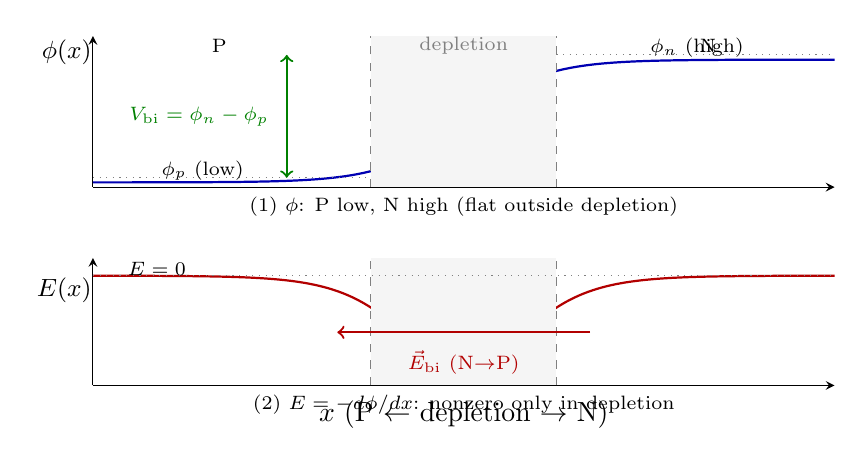
\begin{tikzpicture}
  \def\Vbi{0.52}
  \def\Wdep{0.48}

  % --- top: potential phi(x) ---
  \begin{axis}[
    name=phiaxis,
    width=11cm,
    height=3.5cm,
    xmin=-2.2, xmax=2.2,
    ymin=-0.02, ymax=0.62,
    axis lines=left,
    xtick=\empty,
    ytick=\empty,
    clip=false,
  ]
    \addplot[blue!70!black, thick, domain=-2.2:2.2, samples=250]
      {0.5*\Vbi*(tanh(x/\Wdep)+1)};

    \draw[dashed, gray] (axis cs:-0.55,-0.02) -- (axis cs:-0.55,0.62);
    \draw[dashed, gray] (axis cs:0.55,-0.02) -- (axis cs:0.55,0.62);
    \fill[gray!8] (axis cs:-0.55,-0.02) rectangle (axis cs:0.55,0.62);

    \node[font=\scriptsize] at (axis cs:-1.45,0.58) {P};
    \node[font=\scriptsize] at (axis cs:1.45,0.58) {N};
    \node[font=\scriptsize, gray] at (axis cs:0,0.58) {depletion};

    \node[font=\small, anchor=east] at (axis cs:-2.15,0.55) {$\phi(x)$};

    % flat levels (match curve)
    \draw[dotted, gray] (axis cs:-2.2,0.02) -- (axis cs:-0.55,0.02);
    \draw[dotted, gray] (axis cs:0.55,0.54) -- (axis cs:2.2,0.54);
    \node[font=\scriptsize, anchor=west] at (axis cs:-1.85,0.05) {$\phi_p$ (low)};
    \node[font=\scriptsize, anchor=west] at (axis cs:1.05,0.57) {$\phi_n$ (high)};

    \draw[<->, thick, green!50!black] (axis cs:-1.05,0.02) -- (axis cs:-1.05,0.54);
    \node[font=\scriptsize, green!50!black, anchor=east] at (axis cs:-1.1,0.28)
      {$V_{\mathrm{bi}}=\phi_n-\phi_p$};

    \node[font=\scriptsize, anchor=north, align=center] at (axis cs:0,-0.02)
      {(1) $\phi$: P low, N high (flat outside depletion)};
  \end{axis}

  % --- bottom: E(x) = -d phi/dx ---
  \begin{axis}[
    at={(phiaxis.south west)},
    anchor=north west,
    yshift=-0.9cm,
    width=11cm,
    height=3.2cm,
    xmin=-2.2, xmax=2.2,
    ymin=-0.62, ymax=0.1,
    axis lines=left,
    xlabel={$x$ (P $\leftarrow$ depletion $\rightarrow$ N)},
    xtick=\empty,
    ytick=\empty,
    clip=false,
  ]
    \addplot[red!70!black, thick, domain=-2.2:2.2, samples=250]
      {-0.5*\Vbi/\Wdep*(1/cosh(x/\Wdep))^2};

    \draw[dashed, gray] (axis cs:-0.55,-0.62) -- (axis cs:-0.55,0.1);
    \draw[dashed, gray] (axis cs:0.55,-0.62) -- (axis cs:0.55,0.1);
    \fill[gray!8] (axis cs:-0.55,-0.62) rectangle (axis cs:0.55,0.1);

    \draw[dotted, gray] (axis cs:-2.2,0) -- (axis cs:2.2,0);
    \node[font=\scriptsize, anchor=west] at (axis cs:-2.05,0.04) {$E=0$};

    \node[font=\small, anchor=east] at (axis cs:-2.15,-0.08) {$E(x)$};

    \draw[->, thick, red!70!black] (axis cs:0.75,-0.32) -- (axis cs:-0.75,-0.32)
      node[midway, below=3pt, font=\scriptsize] {$\vec{E}_{\mathrm{bi}}$ (N$\to$P)};

    \node[font=\scriptsize, anchor=north, align=center] at (axis cs:0,-0.62)
      {(2) $E=-d\phi/dx$: nonzero only in depletion};
  \end{axis}

\end{tikzpicture}
\end{document}
